\documentclass[12pt,a4paper]{article}
\usepackage[utf8]{inputenc}
\usepackage[T1]{fontenc}
\usepackage{amsmath}
\usepackage{textcomp}

\usepackage{geometry}
\geometry{a4paper,left=25mm,right=25mm, top=2cm, bottom=2cm} 

\usepackage{graphicx} %fuer bilder

\usepackage{verbatim}


\usepackage{placeins}

 \usepackage{mathptmx}
 \usepackage[scaled=.90]{helvet}
 \usepackage{courier}

\usepackage{enumitem}

\usepackage{listings}
\usepackage{color}
 
\definecolor{dkgreen}{rgb}{0,0.6,0}
\definecolor{gray}{rgb}{0.5,0.5,0.5}
\definecolor{mauve}{rgb}{0.58,0,0.82}

\pagestyle{empty}
\lstset{numbers=left,language=C++}
\lstset{showstringspaces=false,
basicstyle=\ttfamily\footnotesize,
breaklines=true,
tabsize=3,
commentstyle=\color{dkgreen},      % comment style
inputencoding={ansinew},
title=\lstname %zeigt titel der datei an
}

\usepackage{pdfpages}% fuer pdfs



%keine einrückungen bei absatz
\parindent 0pt

\begin{document}
\title{SPV Projekt}
\author{Reinhard Penn, Bernhard Selymes}
\date{May 2015}

\normalsize

%Pfad zu c++ Dateien


%Beginn des Dokuments

\newcommand{\Uebung}{SensorValues}
\newcommand{\srcpath}{../../src}
\newcommand{\screens}{./Screenshots}

%Angabe
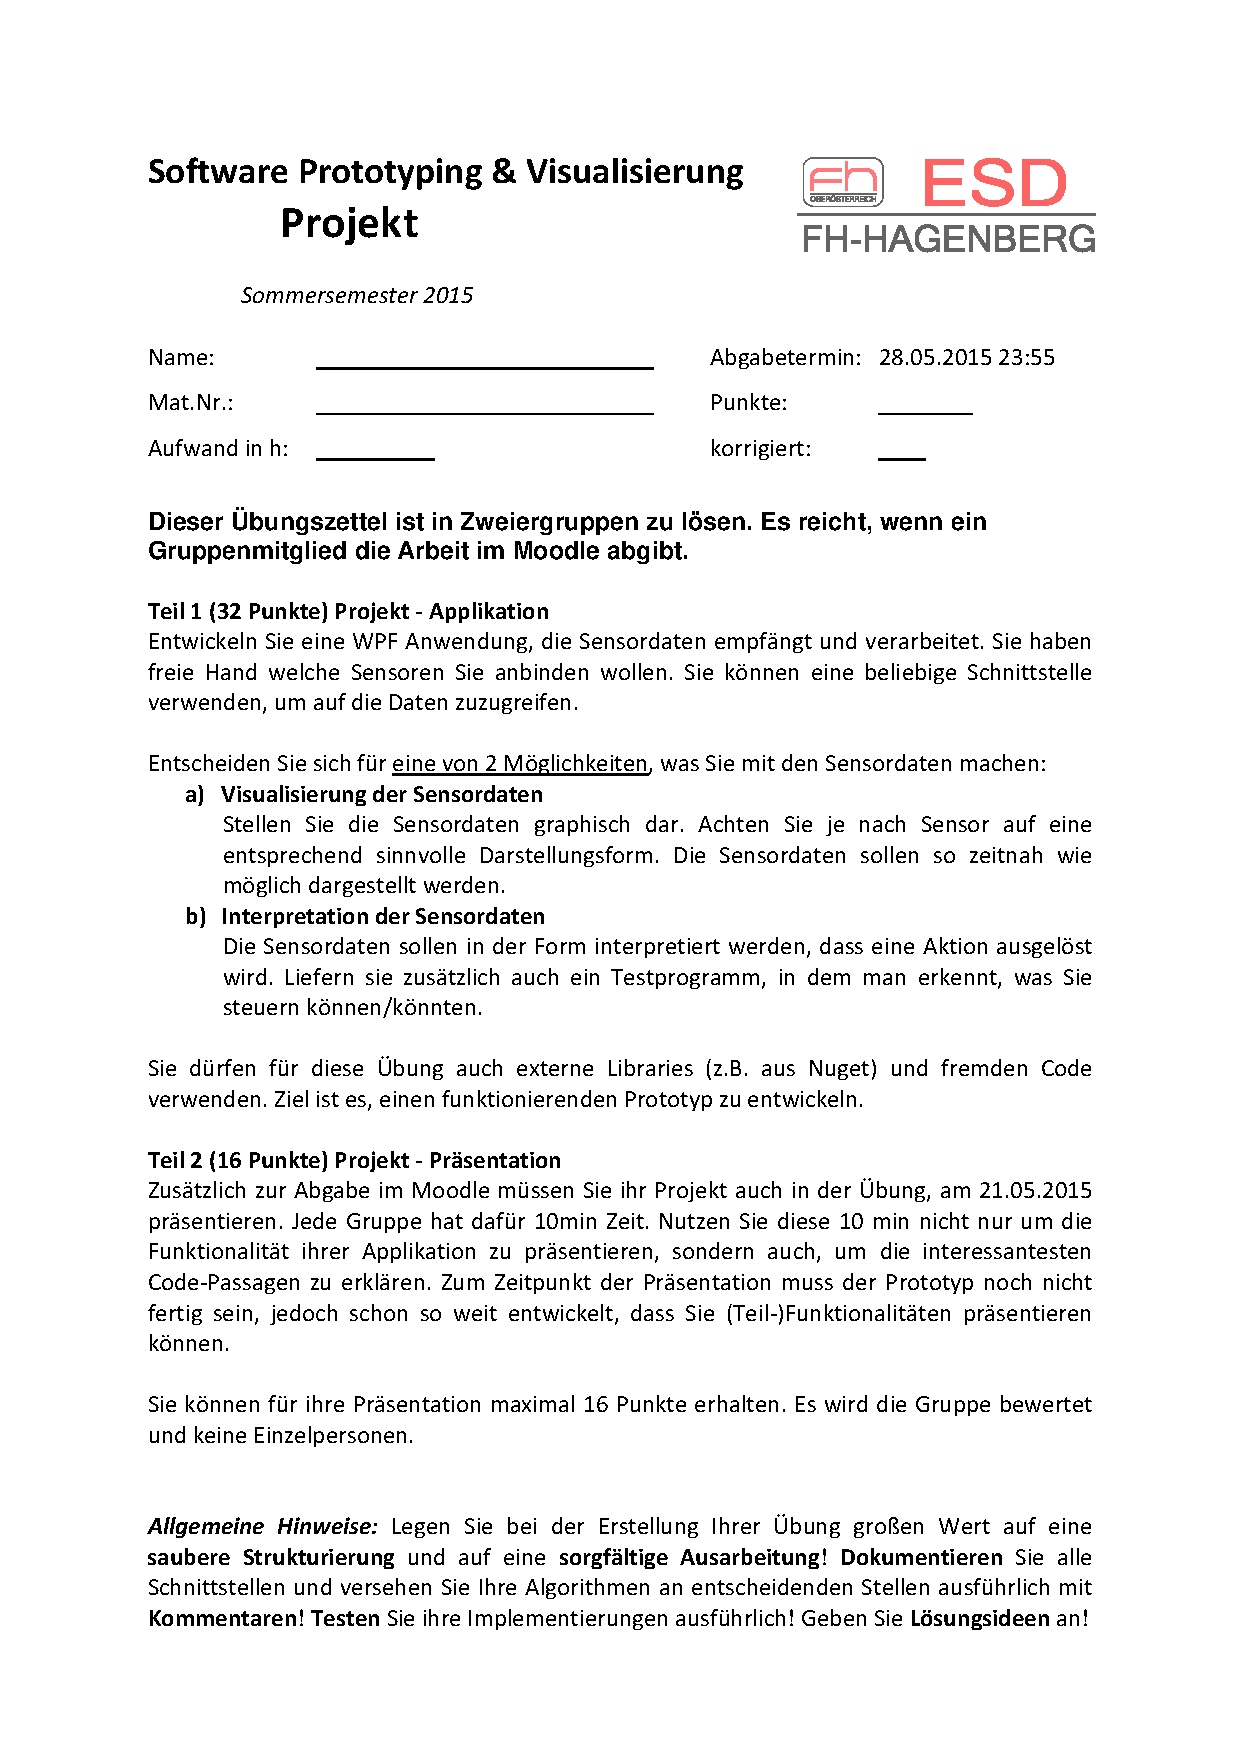
\includepdf[pages=-]{../Angabe.pdf}

\section{Dokumentation}

\subsection{Server Client Kommunikation}
Die Kommunikation basiert auf TCP/IP. Kommuniziert wird zwischen einem Server (WPF App) und einem Client (Android App oder C\# Testclient). Die Daten werden in XML-Format geschickt.
Das Format wird durch eine Klasse, die die Sensorwerte beinhaltet, bestimmt. Diese Klasse wird verwendet um die Daten in XML zu serialisieren bzw. zu deserialisieren.

\subsection{Android App}
Die Android App hat folgende Bedienelemente:
\begin{itemize}[noitemsep]
	\item Feld für Server IP Adresse
	\item Feld für Server Port
	\item Connect Button
	\item Disconnect Button
	\item Feld für Anzeige der Sensorwerte
\end{itemize}

Mithilfe eines Sensor Managers werden die Sensordaten des Androidgerätes in periodischen Abständen ausgelesen. Welcher Sensor ausgelesen werden soll, kann eingestellt werden. Es können auch mehrere Sensoren ausgelesen werden.

\subsection{WPF App}
Die WPF App hat folgende Elemente:
\begin{itemize}[noitemsep]
	\item Ip Adresse des Servers
	\item Port des Servers
	\item Start Button
	\item Stop Button
	\item Anzeige eines 3D Objektes
\end{itemize}

In einem Backgroundworker läuft ein Server welcher auf Daten von einem Client wartet. Sobald Daten vorhanden sind werden die entsprechenden Properties, welche and die GUI gebunden sind (zum Beispiel Winkelwerte), gesetzt. Die 3D Darstellung des Androidgerätes wurden mit einem ModelVisual3D in einem Viewport realisiert.

\subsection{C\# Testclient}
Zusätzlich zur Android App wurde für Testzwecke ein C\# Testclient entwickelt. Dieser schickt in einem einstellbaren Intervall zufällige Testwerte an den Server.

\subsection{Erweiterbarkeit}
In der Android App können beliebige Sensorwerte ausgelesen werden. Die Klasse für die Sensordaten muss entsprechend verändert werden. In der WPF Applikation können weitere Tabs hinzugefügt werden in denen dann verschiedene Sensordaten (z.B. Temperatur als Thermometer oder Lichteinfall als Lampe, ...) visualisiert werden können.

\newpage
\section{Test und Screenshots}

\begin{figure}[!htb]%
\centering
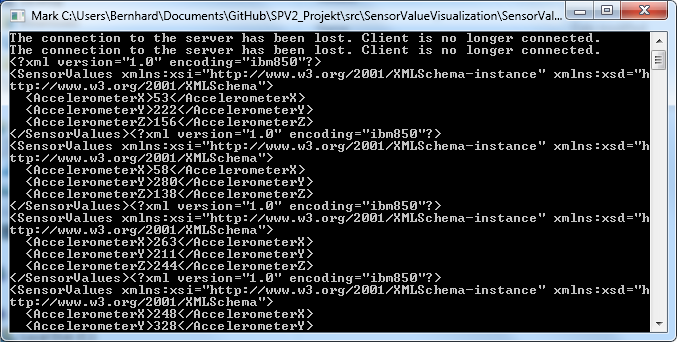
\includegraphics[scale=0.5]{\screens/CSharpTestclient.png}%
\caption{C\# Testclient}%
\label{}%
\end{figure}

\begin{figure}[!htb]%
\centering
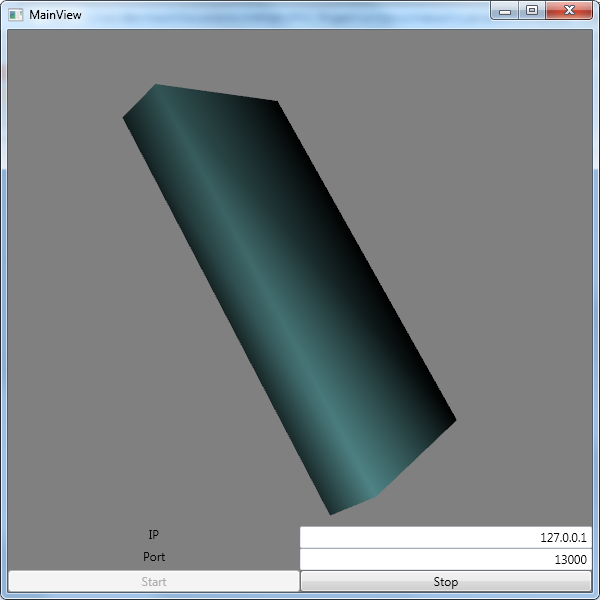
\includegraphics[scale=0.5]{\screens/WPFApp.png}%
\caption{WPF App mit C\# Testclient}%
\label{}%
\end{figure}



\begin{figure}[!htb]%
\centering
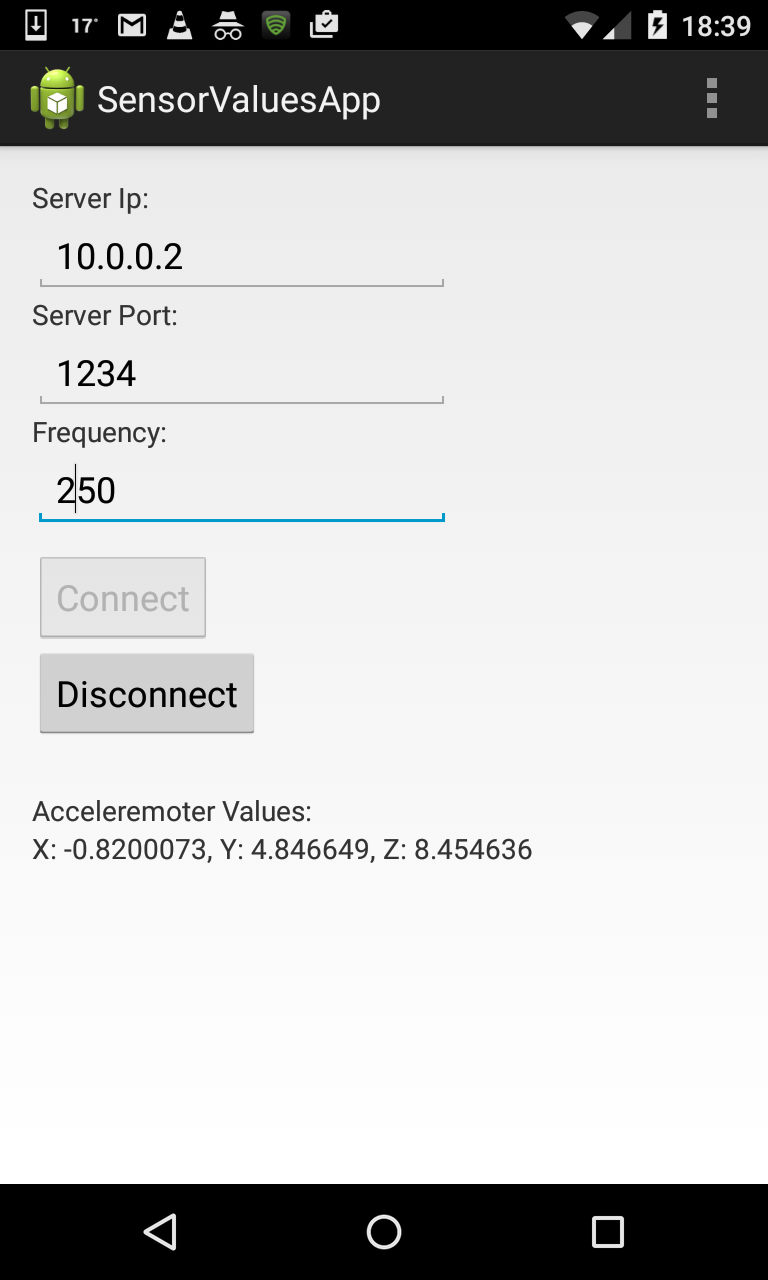
\includegraphics[scale=0.5]{\screens/AndroidApp.png}%
\caption{Android App}%
\label{}%
\end{figure}

\begin{figure}[!htb]%
\centering
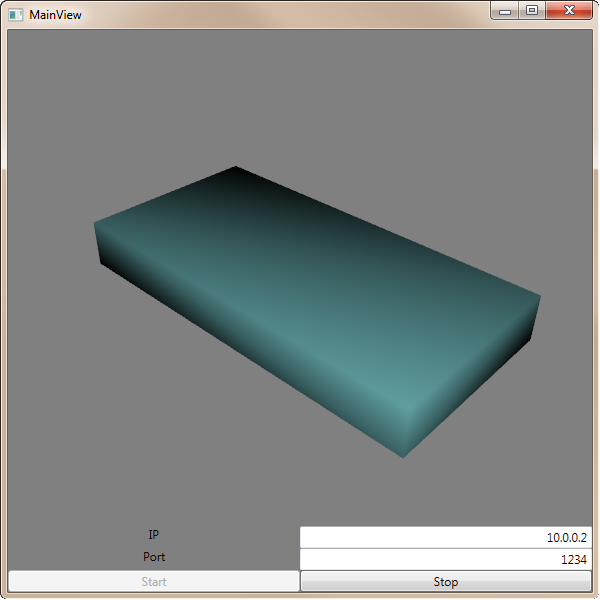
\includegraphics[scale=0.5]{\screens/Test1.png}%
\caption{WPF App Test mit Android App (1)}%
\label{}%
\end{figure}

\begin{figure}[!htb]%
\centering
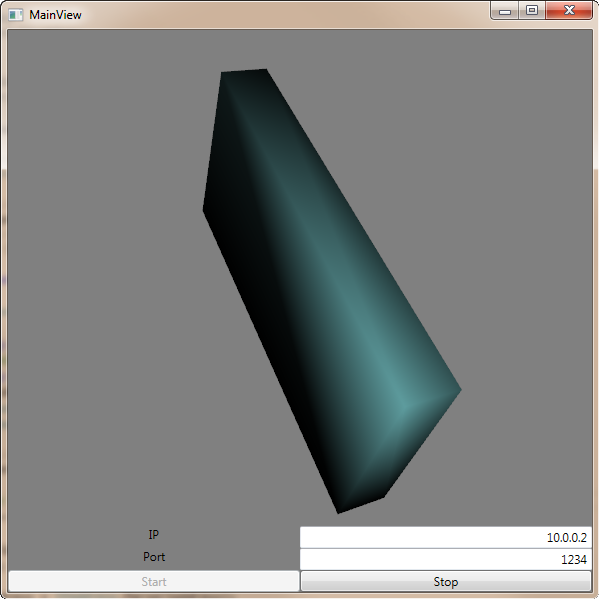
\includegraphics[scale=0.5]{\screens/Test2.png}%
\caption{WPF App Test mit Android App (2)}%
\label{}%
\end{figure}

\FloatBarrier
\newpage
\section{Source Code}

\subsection{WPF App}
C\# Klasse für Sensordaten:
\lstinputlisting{\srcpath/SensorValueVisualization/SensorValues/SensorValues.cs}

WPF App:
\lstinputlisting{\srcpath/SensorValueVisualization/SensorValueVisualization/View/MainView.xaml}

Viewmodel:
\lstinputlisting{\srcpath/SensorValueVisualization/SensorValueVisualization/ViewModel/MainViewModel.cs}

Server:
\lstinputlisting{\srcpath/SensorValueVisualization/SensorValueVisualization/ViewModel/SensorValuesServer.cs}

C\# Testclient:
\lstinputlisting{\srcpath/SensorValueVisualization/SensorValuesTestClient/Program.cs}

\subsection{Android App}
Sensordaten Klasse:
\lstinputlisting[language=Java]{\srcpath/SensorValuesApp/app/src/main/java/reinhard/sensorvaluesapp/SensorValues.java}

TCP Client:
\lstinputlisting[language=Java]{\srcpath/SensorValuesApp/app/src/main/java/reinhard/sensorvaluesapp/TcpClient.java}

Android App:
\lstinputlisting[language=Java]{\srcpath/SensorValuesApp/app/src/main/java/reinhard/sensorvaluesapp/SensorValuesActivity.java}

Android Oberfläche:
\lstinputlisting[language=XML]{\srcpath/SensorValuesApp/app/src/main/res/layout/activity_sensor_values.xml}

XML-Serializer:
\lstinputlisting[language=Java]{\srcpath/SensorValuesApp/app/src/main/java/reinhard/sensorvaluesapp/XmlCreator.java}


\end{document}
